
\section{Diffraction of Light Through a Single Slit}

\makelabheader %(Space for student name, etc., defined in master.tex)

\textbf{Objective}

\begin{itemize}
\item To investigate the diffraction of light waves passing through
a single, narrow slit. 
\end{itemize}
\textbf{Apparatus}

\begin{itemize}
\item Basic optics diode laser
\item Optical bench with rotary motion sensor
\item Phototransistor for measuring light intensity (mounted on rotary motion sensor)
\item ``Single Slit Set'' slit accessory
\item ``Multiple Slit Set'' slit accessory
\item Small plastic ruler
%\item Glass plate with sets of narrow slits
\item {\it DataStudio} 750 Interface
\end{itemize}
\textbf{Introduction}

\textbf{Activity 1: Making Predictions and Taking Data}

(a) In the previous lab, you saw that laser light emitted from two slits can interfere with each other.  If you shine laser light through a single slit, do you predict that you will see any evidence of constructive or destructive interference?  Why or why not?
\answerspace{0.8in}


Well, let's try it!  The setup for this experiment is exactly the same as that for Lab \ref{interference_lab},  but instead of a double slit, you will use the ``Single Slit Set'' slit accessory.  Place it on the optical bench about 70 cm away from the detector, and select the slit with a width of $a = 0.16$ mm.   Set the gain switch to 100 and use the aperture marked ``3''.   Start the program interference.ds and use the computer to take data on the intensity as a function of position by moving the detector slowly across the series of bright spots.  

Your goal is to get as large a signal as you can without having the intensity pinned at its maximum value.  (If the peaks on your graph appear perfectly flat on top, that's probably what's happening.) You may need to adjust either the gain of your detector or the size of its aperture.

(b) In the space below, draw a good, careful graph showing the ``diffraction pattern'' you see.  
Be sure to label your axes!
\answerspace{1.5in}

\pagebreak[2]
\textbf{What's Going On?}

The complex pattern of maxima and minima that you see doesn't look anything like a simple shadow of the single slit.  In fact, it looks a little bit like the kind of interference pattern you get from shining light through two narrow slits.  But what's with that?  How can you have interference from only one slit?

Although there is only one slit, light still comes from many different places \textit{within} the slit: the middle, the left side, the right side, or anywhere in between.  In fact, we could draw an \textit{infinite} number of rays coming from all locations, and going in all directions.  But as before, we'll consider rays traveling only in one particular direction $\theta$ at a time.  The drawing below shows eight evenly spaced rays, numbered 1 through 8.  The gray area in the figure represents all of the infinite rays of light in that direction.

\answerspace{0.2in}
\begin{center}
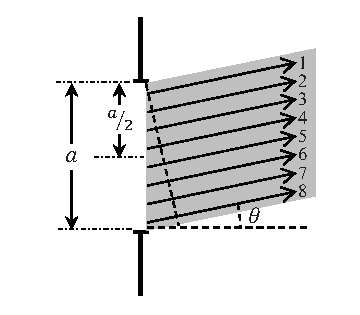
\includegraphics[width=0.4\textwidth]{diffraction_of_light/one_slit.eps}
\end{center}
\answerspace{0.2in}

(c) For a particular angle $\theta$ where the path difference between rays 1 and 5 is given by $\Delta r_{15}=\frac{1}{2}\lambda$, will rays 1 and 5 interfere \textit{CON-structrively} or \textit{DE-structively}?
\answerspace{0.4in}

(d) For an angle $\theta$ where $\Delta r_{15}=\frac{1}{2}\lambda$, what is $\Delta r_{26}$?  What about $\Delta r_{37}$? And $\Delta r_{48}$?
\answerspace{0.5in}

(e) At the particular angle $\theta$ where $\Delta r_{15}=\frac{1}{2}\lambda$, will the intensity at the screen be a maximum, zero, or something in between?
\answerspace{0.4in}

(f) What is $\Delta r_{15}$ in terms of $a$ and $\theta$?
\answerspace{0.4in}

The upshot of this is is that for a single slit, you should have an intensity minimum, with complete destructive interference, at the particular angle $\theta$ where $\frac{a}{2} \sin \theta = \frac{1}{2}\lambda$.  Next, we'll see if there are other angles for which that's also true.

\pagebreak[3]
\textbf{Activity 2: Finding All Intensity Minima}

\vspace{-0.2in}
\begin{center}
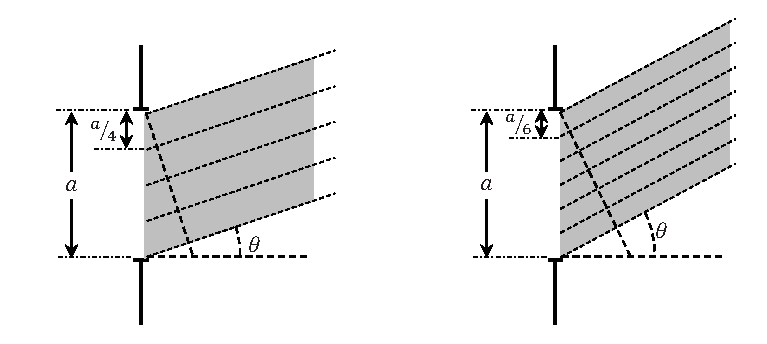
\includegraphics[width=0.7\textwidth]{diffraction_of_light/fourths_and_sixths.eps}
\end{center}
\vspace{-0.2in}

(a) Looking at the left diagram above, write a condition for when the top-most ray will interfere destructively with the ray $\frac{a}{4}$ from the top.  Your equation should be in terms of $a$, $\theta$, and $\lambda$.  
\answerspace{0.4in}

(b) Considering \textit{all} rays at that angle $\theta$, will your condition lead to an intensity minimum with complete destructive interference?
\answerspace{0.4in}

(c) Looking at the right diagram above, write a condition for when the top-most ray will interfere destructively with the ray $\frac{a}{6}$ from the top.  (Again, in terms of $a$, $\theta$, and $\lambda$.)  Will this condition also lead to an overall intensity minimum?
\answerspace{0.4in}

(d) It looks like you could keep dividing the slit into any even number of sections and get the same result.  Write a generalized version of your condition for an intensity minimum in terms of an arbitrary integer $m$.  (You can cancel out a two to simplify your result.)

\answerspace{0.1in}
\hspace{0.8in}\textbf{For a single slit of width \textit{a}, intensity \textit{minima} occur where: }
\answerspace{0.1in}

(e) Is your expression true for $m=0$?
\answerspace{0.4in}

(f) The diffraction pattern for a single slit is shown below.  Label all of the minima with the corresponding value $m=1$, $m=2$, etc.  

%\vspace{-0.2in}
\begin{center}
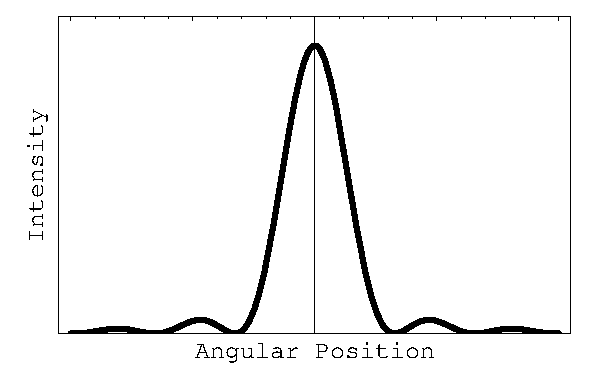
\includegraphics[width=0.4\textwidth]{diffraction_of_light/diffraction_of_light_fig_3.eps}
\end{center}
%\vspace{-0.2in}

\pagebreak[3]

(g) Calculate the angular separation $\theta$ between the central maximum and any numbered minimum you choose in your data, using measurements of $L$ and $\Delta x$ for that minimum.  Use your value for $\theta$ and your expression in part (d) to calculate the width $a$ of the slit.  (The wavelength of the light from your laser is 650 nm.  To get $\theta$, you'll need to measure the distance from the slit to the detector and do some calculations.)    Does your value of $a$ agree with what is written on the slit?
\answerspace{1.0in}


\textbf{Activity 3: What About Intensity Maxima?}

The diagram below shows what happens when all of the rays in a single direction don't neatly divide into an even number of groups that cancel each other out.

\vspace{-0.2in}
\begin{center}
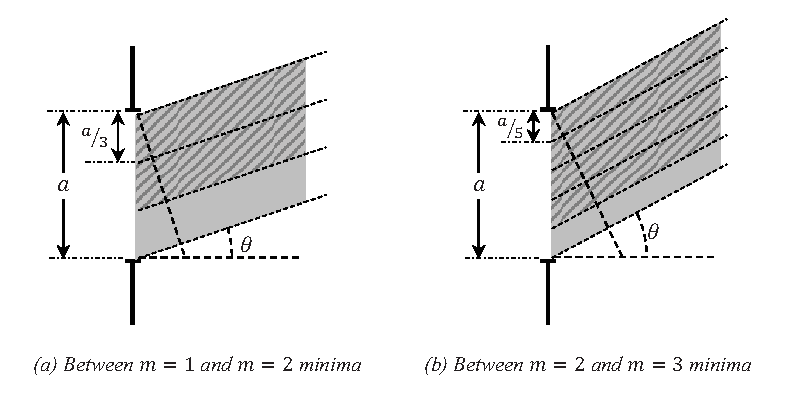
\includegraphics[width=0.7\textwidth]{diffraction_of_light/diffraction_maxima.eps}
\end{center}
\vspace{-0.2in}

The diagram on the left shows rays at an angle $\theta$ where $\frac{a}{3} \sin \theta = \frac{\lambda}{2}$.  In the upper shaded area of the diagram, each ray can be \textit{paired up} with another one exactly $180^{\circ}$ out of phase, so that all of the rays inside that shaded area cancel each other out.  The intensity at the screen or the detector  comes from the unpaired rays that aren't shaded out.

(a) If $\theta$ were \textit{just a little} smaller than what's shown in the left diagram, would the resulting intensity \textit{increase}, \textit{decrease}, or \textit{stay the same}? (Hint: Would there be more or fewer unpaired rays?)
\answerspace{0.4in}

(b) If $theta$ were \textit{just a little} bigger than what's shown in the diagram, would the resulting intensity \textit{increase}, \textit{decrease}, or \textit{stay the same}?  (Hint: would all of the rays in the lower portion remain unpaired?)
\answerspace{0.4in}

(c) The particular $\theta$ shown in the diagram on the left is a maximum in the diffraction pattern.  Is the intensity of that maximum \textit{greater than}, \textit{less than}, or \textit{equal to} the intensity of the maximum at $\theta = 0$?  Why?
\answerspace{0.4in}

(d) Is the intensity of the maximum shown in the diagram on the right \textit{greater than}, \textit{less than}, or \textit{equal to} the intensity of the maximum shown on the left?  Why?  
\answerspace{0.4in}

(e) Do your answers for the last two questions agree with the data you took for the single slit diffraction pattern?
\answerspace{0.2in}


\pagebreak[2]
Although the derivation goes beyond the scope of this course, the intensity $I_{\rm{diff}}$ for the diffraction of a single slit can actually be written in closed form as
\begin{displaymath} 
I_{\rm{diff}} = I_{\rm{max}} \left( \frac {\sin \left(\frac {\pi a} {\lambda} \sin \theta \right)} {\frac {\pi a} {\lambda} \sin \theta} \right)^2 \end{displaymath}

where $a$ is the width of the single slit, \( \theta  \) is the angular
position of the phototransistor relative to the incident beam, and $I_{\rm{max}}$
is the maximum intensity at the center of the diffraction pattern.

\pagebreak[2]
\textbf{Activity 4: Two-Slit Interference Revisited}

(a) Replace the single slit with the ``Multiple Slit Set'' slit accessory, and select the pair of two slits with separation $d=0.125$ mm and width $a=0.04$ mm, labeled with the number ``2''.  Get some good clean data on the intensity $I$ \textit{vs.}~position.

(b) As we described it in Lab \ref{interference_lab}, the interference pattern you see occurs because as the angle $\theta$ increases from zero, the path difference $\Delta r$ between rays from the two slits grows.  Because $\Delta r$ is sometimes an integer multiple of $\lambda$ and sometimes a half-integer multiple of $\lambda$, the intensity oscillates between a maximum (constructive interference) and a minimum (destructive interference).  But if that were all that were going on, your interference pattern would be a simple periodic function with all maxima at exactly the same intensity.  Is that actually what you see?
\answerspace{0.4in}

(c) In fact, you probably see something like the figure below, with some large maxima near the center, and several other much smaller maxima on either side.  (If you didn't see this, try increasing your signal strength, or consult your instructor.)

\vspace{-0.1in}
\begin{center}
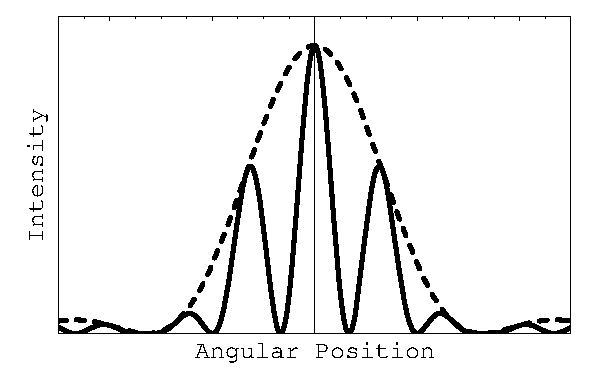
\includegraphics[width=0.4\textwidth]{diffraction_of_light/diffraction_of_light_fig_4.eps}
\end{center}
\vspace{-0.1in}

The reason for the more complicated pattern is that in addition to the interference between rays from the two different slits, each individual slit has a nonzero width $a$, so there's also interference between different rays coming from the \textit{same} slit.  Essentially, there's no way to get big CON-structive interference between the two slits at an angle $\theta$ where all the rays from one slit have canceled each other out.  As a result, the complicated pattern you see is basically the simple oscillating function of two slit interference multiplied by the intensity at that angle from a single slit: 
\begin{displaymath} 
I_{\rm{total}} = I_{\rm{max}} \cos^2 \left (\frac {\pi d} {\lambda} \sin \theta \right) \left(\frac {\sin \left (\frac {\pi a} {\lambda} \sin \theta \right )} {\frac {\pi a} {\lambda} \sin \theta} \right)^2 \end{displaymath}

(d) Looking at your data, identify the position at which the interference maxima  are reduced to zero by the $m=1$ minimum of the single slit diffraction pattern.  Use that angle to calculate the apparent width $a$ of the slits.  Is it consistent with what is written on the slits?
\answerspace{1in}
